%!TEX root=ast2016.tex

\begin{figure*}[t]
  \centering
  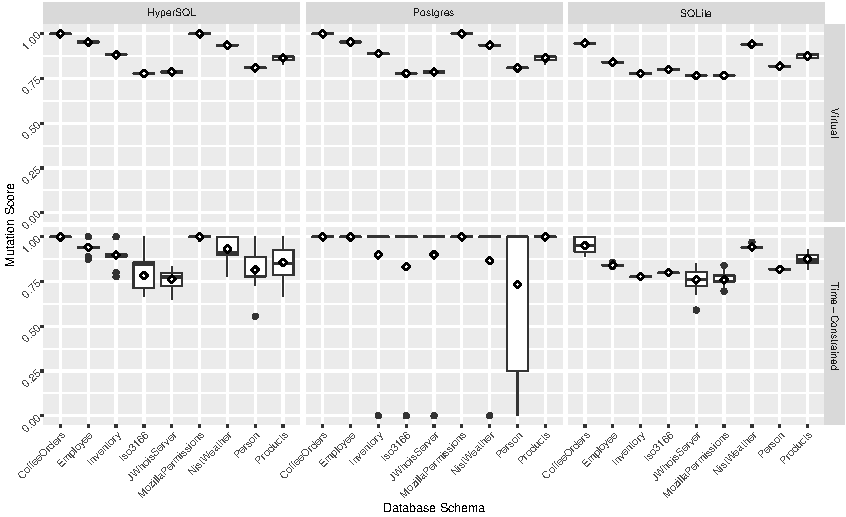
\includegraphics[scale=1.0]{graphics/graphic_bwplot_schema_mutationscore_vm_tcm.pdf}
  \caption{Box plot of the mutation score for the virtual and time-constrained mutation analysis techniques.}
  \label{fig:graphic_bwplot_schema_mutationscore_vm_tcm}

  % NOTE: There is no need to duplicate the content that describes the meaning of the box plot's elements. So, this
  % subcaption explains more about the configuration of the experiment that produced this graph, which is useful.

  % The time-constrained approach was allowed to analyze mutants for as long as the virtual mutation method would have run
  % for the corresponding schema.

  {\small \justifying{ \noindent The meaning of this box plot's elements is the same as the meaning of those described
      in the subcaption of Figure~\ref{fig:graphic_bwplot_schema_analysistime_org_vm}. Additionally, in this box plot a
      filled circle denotes an outlier and the open diamond is the mean value. Using test suites from thirty separate
      runs of the search-based test data generation method developed by McMinn et al.\ \cite{McMinn2015}}, this plot
    shows the variation in the mutation score for both the virtual and the time-constrained method and for all of the
  chosen relational schemas and the three database management systems. \par}

\end{figure*}
